\vspace{-0.5cm}
\section{Introduction}
\vspace{-0.3cm}


High-capacity neural networks trained on large, diverse datasets have led to remarkable 
models that can solve numerous tasks, rapidly adapt to new tasks, and produce general-purpose representations in NLP and vision~\citep{brown2020language,he2111masked}. %in vision~\citep{he2111masked} and NLP~\citep{brown2020language}, 
The promise of offline RL is to leverage these advances to produce  polices with broad generalization, emergent capabilities, and performance that exceeds the capabilities demonstrated in the training dataset. %,
% Offline reinforcement learning (RL) can potentially enable RL methods to leverage broad and diverse sources of previously collected data. Much like how the impressive results in vision~\citep{he2111masked}, and NLP~\citep{brown2020language} have been generally enabled by the use of large datasets in concert with huge models, RL methods that can utilize large, heterogeneous datasets with high-capacity models provide a promising approach to achieve the same sort of broad generalization, emergent capabilities, and high performance for downstream control problems. 
%%AK: first motivate why studying scaling of offline RL is even important and not done
Thus far, the only offline RL approaches that demonstrate broadly generalizing policies and transferable representations are heavily-based on supervised learning~\citep{reed2022generalist,lee2022multi}. However, these approaches are likely to perform poorly when the dataset does not contain expert trajectories~\citep{kumar2021should}.

Offline Q-learning performs well across dataset compositions in a variety of
simulated~\citep{gulcehre2020rl, fu2020d4rl} and real-world domains~\citep{chebotar2021actionable, soarespulserl},
however, these are largely centered around small-scale, single-task problems where broad generalization and learning general-purpose representations is not expected. \emph{Scaling these methods up to high-capcity models on large, diverse datasets is the critical challenge.} 
Prior works hint at the difficulties: on small-scale, single-task deep RL benchmarks, scaling model capacity can lead to instabilities or degrade performance~\citep{van2018deep,sinha2020d2rl,ota2021training} explaining why decade-old tiny 3-layer CNN architectures~\citep{mnih2013playing} are still prevalent. Moreover, works that have scaled architectures to millions of parameters~\citep{espeholt2018impala,teh2017distral, vinyals2019grandmaster,schrittwieser2021online} typically focus on \emph{online} learning and employ many sophisticated techniques to stabilize learning, such as supervised auxiliary losses, distillation, and pre-training. 
Thus, it is unclear whether offline Q-learning can be scaled to high-capacity models.

In this paper, we demonstrate that with careful design decisions, \emph{offline Q-learning can scale} to high-capacity models trained on large, diverse datasets from many tasks, leading to policies that not only generalize broadly, but also learn representations that effectively transfer to new downstream tasks and exceed  the performance in the training dataset. 
Crucially, we make three modifications motivated by prior work in deep learning and offline RL. First, we find that a modified ResNet architecture~\citep{resnet} substantially outperforms typical deep RL architectures and follows a power-law relationship between model capacity and performance, unlike common alternatives. 
Second, a discretized representation of the return distribution with a distributional cross-entropy loss~\citep{bellemare2017distributional}  substantially improves performance compared to standard Q-learning, that utilizes mean squared error. Finally, feature normalization on the intermediate feature representations stabilizes training and prevents feature co-adaptation~\citep{kumar2021dr3}. 


To systematically evaluate the impact of these changes on scaling and generalization, we train a single policy to play 40 Atari games~\citep{bellemare2013arcade, agarwal2019optimistic}, similarly to \citet{lee2022multi}, and evaluate performance when the training dataset contains expert trajectories \emph{and} when the data is sub-optimal. This problem is especially challenging because of the diversity of games with their own unique dynamics, reward, visuals, and agent embodiments. Furthermore, the sub-optimal data setting requires the learning algorithm to ``stitch together'' useful segments of sub-optimal trajectories to perform well. 
To investigate generalization of learned representations, we evaluate offline fine-tuning to \emph{never-before-seen} games and fast online adaptation on new \emph{variants} of training games~(Section~\ref{sec:ft_off_on}).
With our modifications, 
\begin{itemize}
    \item Offline Q-learning learns policies that attain more than 100\% human-level performance on most of these games, about \textbf{2x} better than prior supervised learning~(SL) approaches for learning from sub-optimal offline data (51\% human-level performance). 
    \item Akin to scaling laws in SL~\citep{kaplan2020scaling}, offline Q-learning performance scales favorably with model capacity~(Figure~\ref{fig:scaling}). 
    \item Representations learned by offline Q-learning give rise to more than 80\% better performance when fine-tuning on new games compared to representations from state-of-the-art return-conditioned supervised~\citep{lee2022multi} and self-supervised methods~\citep{he2111masked,oord2018representation}. 
\end{itemize}
By scaling Q-learning, we realize the promise of offline RL: learning policies that broadly generalize and exceed the capabilities demonstrated in the training dataset. We hope that this work encourages large-scale offline RL applications, especially in domains with large sub-optimal datasets.

\begin{figure}[t]
    \centering
    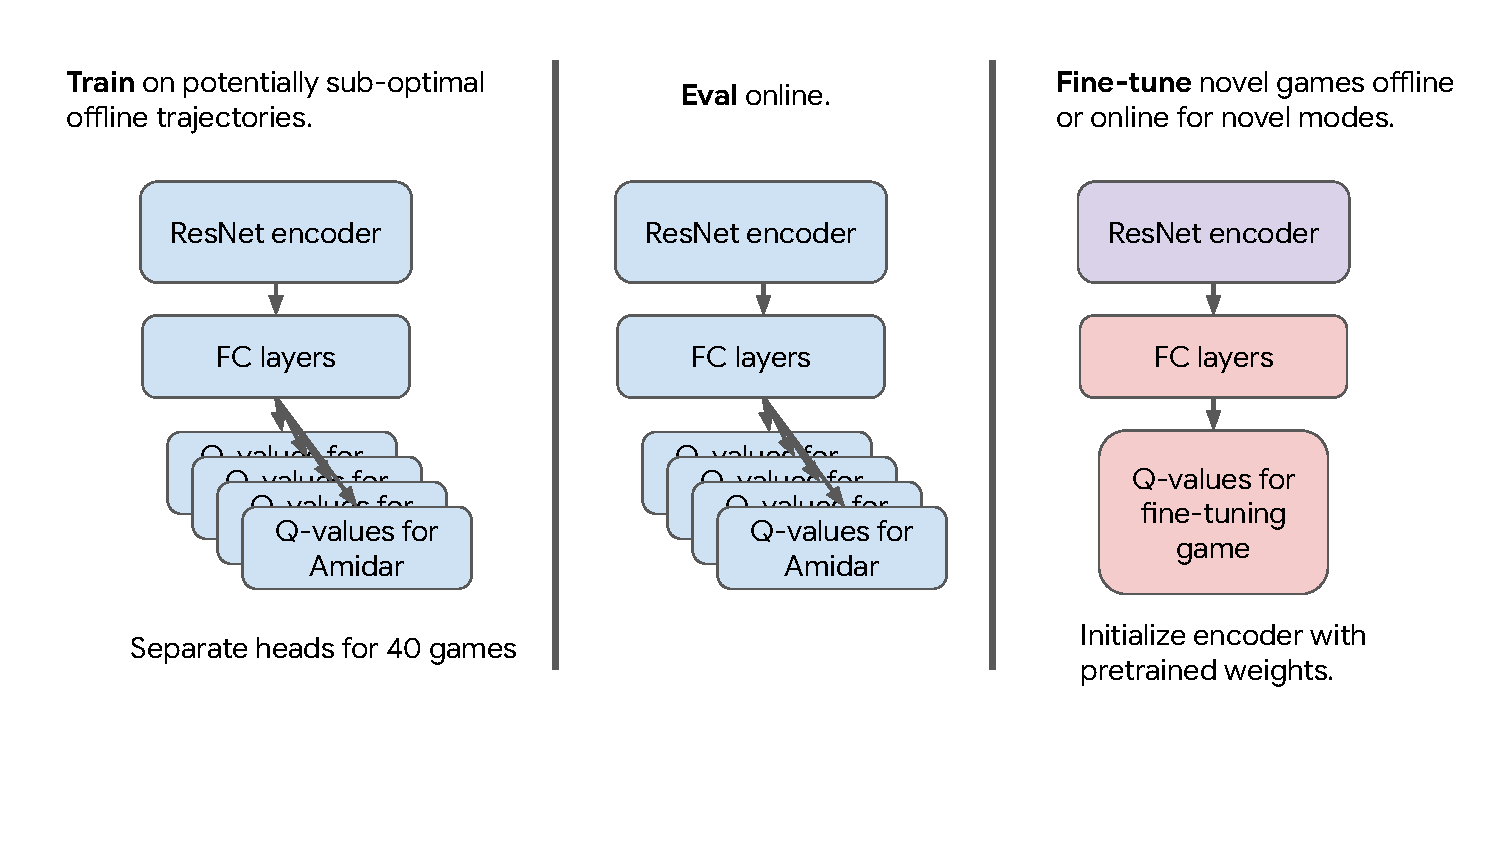
\includegraphics[width=0.75\linewidth]{iclr2023/figures/fig_overview.pdf}
    \vspace{-0.3cm}
    \caption{\footnotesize{An overview of the training and evaluation setup. Models are trained offline with potentially sub-optimal data. We adapt CQL to the multi-task setup via a multi-headed architecture. The pre-trained visual encoder is reused in fine-tuning (the weights are either frozen or fine-tuned), whereas the downstream fully-connected layers are reinitialized and trained.}}
    \label{fig:overview}
    \vspace{-0.5cm}
\end{figure}


\vspace{-0.1cm}
\begin{figure}[t]
    \centering
    
\includegraphics[width=0.95\linewidth]{iclr2023/figures/training_fig_legend_20p.pdf}
    \vspace{-0.1cm}
    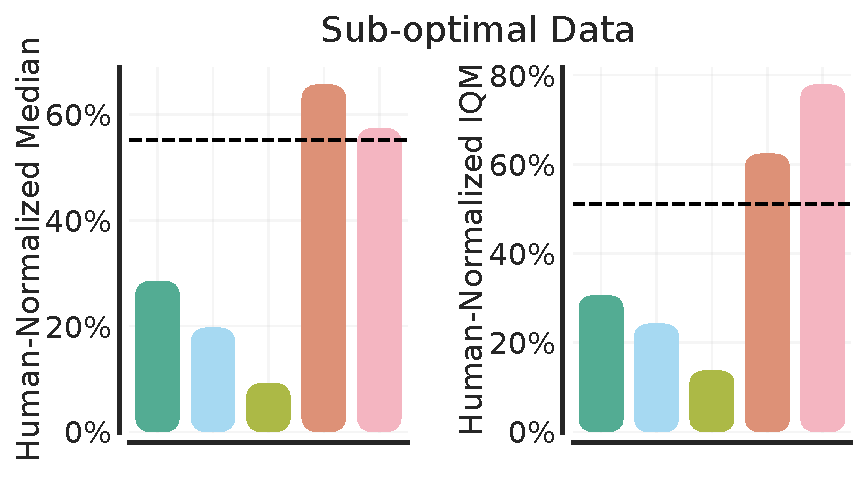
\includegraphics[width=0.48\linewidth]{iclr2023/figures/suboptimal_data_results.pdf}
    ~~~
    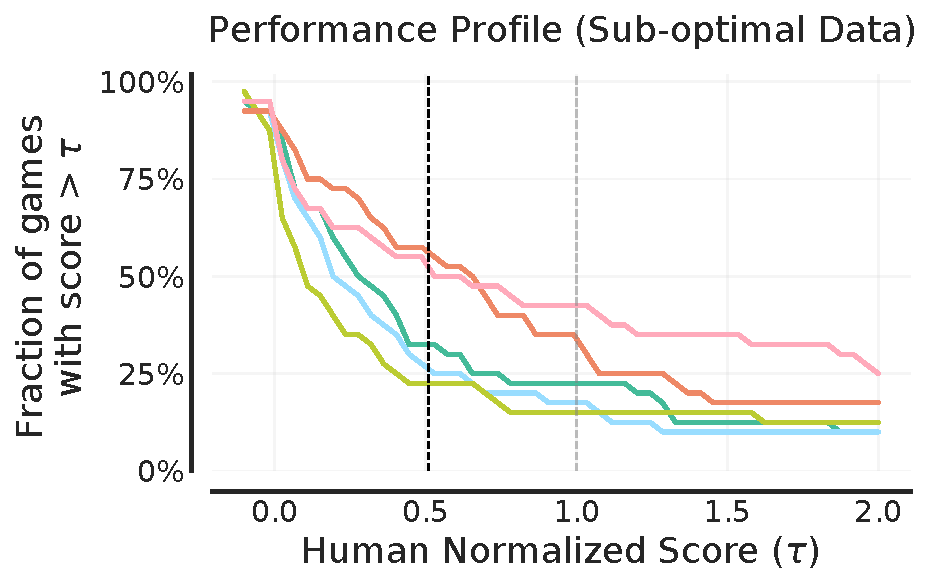
\includegraphics[width=0.45\linewidth]{iclr2023/figures/perf_profile_20p.pdf}
    \vspace{-0.3cm}
    \caption{\footnotesize{Offline multi-task performance on 40 games with sub-optimal data. \textbf{Left}. Scaled QL significantly outperforms the previous state-of-the-art method, DT, attaining about a \textbf{2.5x} performance improvement in normalized IQM score. To contextualize the absolute numbers, we include online multi-task Impala DQN~\citep{espeholt2018impala} trained on 5x as much data.
    \textbf{Right}. Performance profiles~\citep{agarwal2021deep} showing the distribution of normalized scores across all 40 training games (higher is better). 
    Scaled QL stochastically dominates other offline RL algorithms and achieves superhuman performance in 40\% of the games. ``Behavior policy'' corresponds to the score of the dataset trajectories. {Online MT DQN (5X), taken directly from \citet{lee2022multi}, corresponds to running multi-task online RL for 5x more data with IMPALA (details in Appendix~\ref{sec:online_mt_dqn}).}}}
    \label{fig:suboptimal_offline}
    \vspace{-0.3cm}
\end{figure}
